\documentclass{article}
\usepackage{graphicx} % Extended graphics inclusions
\usepackage{float}
\usepackage{url} % For \url{}
\usepackage{../config/atxy} % For front cover
\usepackage{amsfonts} % Needed for some fonts
\usepackage[usenames]{color} % Needed for colored R input/output
\usepackage{pdfcolmk} % Correct some problems with the color stack


\title{Multivariate analyses}
\author{Lobry, J.R.}

\usepackage{Sweave}
\begin{document}
%
% To change the R input/output style:
%
\definecolor{Soutput}{rgb}{0,0,0.56}
\definecolor{Sinput}{rgb}{0.56,0,0}
\DefineVerbatimEnvironment{Sinput}{Verbatim}
{formatcom={\color{Sinput}},fontsize=\footnotesize, baselinestretch=0.75}
\DefineVerbatimEnvironment{Soutput}{Verbatim}
{formatcom={\color{Soutput}},fontsize=\footnotesize, baselinestretch=0.75}
%
% This removes the extra spacing after code and output chunks in Sweave,
% but keeps the spacing around the whole block.
%
\fvset{listparameters={\setlength{\topsep}{0pt}}}
\renewenvironment{Schunk}{\vspace{\topsep}}{\vspace{\topsep}}
%
% Rlogo
%
\newcommand{\Rlogo}{\protect
\includegraphics[height=1.8ex,keepaspectratio]{../figs/Rlogo.pdf}}
%
% Shortcut for seqinR:
%
\newcommand{\seqinr}{\texttt{seqin\bf{R}}}
\newcommand{\Seqinr}{\texttt{Seqin\bf{R}}}
\fvset{fontsize= \scriptsize}
%
% R output options and libraries to be loaded.
%
%
%  Sweave Options
%
% Put all figures in the fig folder and start the name with current file name.
% Do not produce EPS files
%


\maketitle
% BEGIN - DO NOT REMOVE THIS LINE

\section{Correspondence analysis}

This is the most popular multivariate data analysis technique for amino-acid
and codon count tables, its application, however, is not without pitfalls \cite{misuse}.
Its primary goal is to transform a table of counts
into a graphical display, in which each gene (or protein) and each codon (or amino-acid)
is depicted as a point. Correspondence analysis (CA) may be defined as a special 
case of principal components analysis (PCA) with a different underlying metrics.
The interest of the metrics in CA, that is the way we measure the distance between
two individuals, is illustrated bellow with a very simple example (Table \ref{toyaa} inspired from \cite{CG}) with only
three proteins having only three amino-acids, so that we can represent exactly
on a map the consequences of the metric choice.

\begin{Schunk}
\begin{Sinput}
 data(toyaa)
 toyaa
\end{Sinput}
\begin{Soutput}
  Ala Val Cys
1 130  70   0
2  60  40   0
3  60  35   5
\end{Soutput}
\end{Schunk}

% latex table generated in R 2.2.0 by xtable 1.3-0 package
% Thu Dec 22 11:14:23 2005
\begin{table}[ht]
\begin{center}
\begin{tabular}{rrrr}
\hline
 & Ala & Val & Cys \\
\hline
1 & 130 & 70 & 0 \\
2 & 60 & 40 & 0 \\
3 & 60 & 35 & 5 \\
\hline
\end{tabular}
\caption{A very simple example of amino-acid counts in three proteins to be loaded with \texttt{data(toyaa).}}
\label{toyaa}
\end{center}
\end{table}


Let's first use the regular Euclidian metrics between two proteins $i$ and $i'$,
\begin{equation}
d^2(i,i') = \sum_{j=1}^{J}(n_{ij} - n_{i'j})^2
\label{euclidian}
\end{equation}
to visualize this small data set:

\begin{Schunk}
\begin{Sinput}
 library(ade4)
 pco <- dudi.pco(dist(toyaa), scann = F, nf = 2)
 myplot <- function(res, ...) {
     plot(res$li[, 1], res$li[, 2], ...)
     text(x = res$li[, 1], y = res$li[, 2], labels = 1:3, pos = ifelse(res$li[, 
         2] < 0, 1, 3))
     perm <- c(3, 1, 2)
     lines(c(res$li[, 1], res$li[perm, 1]), c(res$li[, 2], 
         res$li[perm, 2]))
 }
 myplot(pco, main = "Euclidian distance", asp = 1, pch = 19, 
     xlab = "", ylab = "", las = 1)
\end{Sinput}
\end{Schunk}
\includegraphics{../figs/multivariate-euclidian}

From this point of view, the first individual is far away from the two others. But
thinking about it, this is a rather trivial effect of protein size:

\begin{Schunk}
\begin{Sinput}
 rowSums(toyaa)
\end{Sinput}
\begin{Soutput}
  1   2   3 
200 100 100 
\end{Soutput}
\end{Schunk}

With 200 amino-acids, the first protein is two times bigger 
than the others so that when computing the Euclidian distance (\ref{euclidian}) its $n_{ij}$ entries
are on average bigger, sending it away from the others.
To get rid of this trivial effect, the first
obvious idea is to divide counts by protein lengths so as to work with 
\emph{protein profiles}. The corresponding distance is,

\begin{equation}
d^2(i,i') = \sum_{j=1}^{J}(\frac{n_{ij}}{n_{i\bullet}} - \frac{n_{i'j}}{n_{i'\bullet}})^2
\label{euclprof}
\end{equation}

where $n_{i\bullet}$ and $n_{i'\bullet}$ are the total number of amino-acids
in protein $i$ and $i'$, respectively.

\begin{Schunk}
\begin{Sinput}
 profile <- toyaa/rowSums(toyaa)
 profile
\end{Sinput}
\begin{Soutput}
   Ala  Val  Cys
1 0.65 0.35 0.00
2 0.60 0.40 0.00
3 0.60 0.35 0.05
\end{Soutput}
\begin{Sinput}
 pco1 <- dudi.pco(dist(profile), scann = F, nf = 2)
 myplot(pco1, main = "Euclidian distance on protein profiles", 
     asp = 1, pch = 19, xlab = "", ylab = "", ylim = range(pco1$li[, 
         2]) * 1.2)
\end{Sinput}
\end{Schunk}
\includegraphics{../figs/multivariate-profile}

The pattern is now completely different with the three protein equally spaced.
This is normal because in terms of relative amino-acid composition they are
all differing two-by-two by $5\%$ at the level of two amino-acids only. We
have clearly removed the trivial protein size effect, but this is still not completely
satisfactory. The proteins are differing by $5\%$ for all amino-acids but the situation 
is somewhat different for \texttt{Cys} because this amino-acid is very rare.
A difference of $5\%$ for a rare amino-acid has not the same significance than
a difference of $5\%$ for a common amino-acid such as \texttt{Ala} in our
example. To cope with this, CA make use of a variance-standardizing
technique to compensate for the larger variance in high frequencies and the 
smaller variance in low frequencies. This is achieved with the use of the 
\emph{chi-square distance} ($\chi^2$) which differs from the previous Euclidean distance 
on profiles (\ref{euclprof}) in that each square is weighted by the inverse of 
the frequency corresponding to each term,

\begin{equation}
d^2(i,i') = n_{\bullet\bullet}\sum_{j=1}^{J}\frac{1}{n_{{\bullet}j}}(\frac{n_{ij}}{n_{i\bullet}} - \frac{n_{i'j}}{n_{i'\bullet}})^2
\label{chi}
\end{equation}

where $n_{{\bullet}j}$ is the total number of amino-acid of kind $j$ and
$n_{\bullet\bullet}$ the total number of amino-acids. With this point
of view, the map is now like this:

\begin{Schunk}
\begin{Sinput}
 coa <- dudi.coa(toyaa, scann = FALSE, nf = 2)
 myplot(coa, main = expression(paste(chi^2, " distance")), 
     asp = 1, pch = 19, xlab = "", ylab = "")
\end{Sinput}
\end{Schunk}
\includegraphics{../figs/multivariate-afc}

The pattern is completely different with now protein number 3 which is far away from
the others because it is enriched in the rare amino-acid \texttt{Cys} as compared to
others.

The purpose of this small example was to demonstrates that the metric choice
is not without dramatic effects on the visualisation of data. Depending on your
objectives, you may agree or disagree with the $\chi^2$ metric choice, that's
not a problem, the important point is that you should be aware that there is
an underlying model there, \textit{chacun a son go{\^u}t} ou 
\textit{chacun {\`a} son go{\^u}t}, it's up to you.

Now, if you agree with the  $\chi^2$ metric choice, there's a nice
representation that may help you for the interpretation of results. 
This is a kind of "biplot" representation in which the lines and
columns of the dataset are simultaneously represented, in the
right way, that is as a graphical \textit{translation} of a 
mathematical theorem, but let's see how does it look like in practice: 

\begin{Schunk}
\begin{Sinput}
 scatter(coa, clab.col = 0.8, clab.row = 0.8, posi = "none")
\end{Sinput}
\begin{Soutput}
NULL
\end{Soutput}
\end{Schunk}
\includegraphics{../figs/multivariate-scatter}

What is obvious is that the Cys content has a major effect on protein
variability here, no scoop. Please note how the information is well
summarised here: protein number 3 differs because it's enriched in
in Cys ; protein number 1 and 2 are almost the same but there is a
small trend protein number 1 to be enriched in Ala. As compared to
to table \ref{toyaa} this graph is of poor information here, so let's
try a more big-rooom-sized example (with $20$ columns so as to
illustrate the dimension reduction technique).

Data are from \cite{lobrygautier}, a sample of the proteome of
\textit{Escherichia coli}. According to the title of this paper,
the most important factor for the between-protein variability is
hydrophilic - hydrophobic gradient. Let's try to reproduce this
assertion :

\begin{Schunk}
\begin{Sinput}
 download.file(url = "ftp://pbil.univ-lyon1.fr/pub/datasets/NAR94/data.txt", 
     destfile = "data.txt")
 ec <- read.table(file = "data.txt", header = TRUE, row.names = 1)
 ec.coa <- dudi.coa(ec, scann = FALSE, nf = 1)
 F1 <- ec.coa$li[, 1]
 hist(F1, proba = TRUE, xlab = "First factor for amino-acid variability", 
     col = grey(0.8), border = grey(0.5), las = 1, ylim = c(0, 
         6), main = "Protein distribution on first factor")
 lines(density(F1, adjust = 0.5), lwd = 2)
\end{Sinput}
\end{Schunk}
\includegraphics{../figs/multivariate-lobrygautier}

There is clearly a bimodal distribution of proteins on the first factor. What are the
the amino-acid coordinates on this factor?

\begin{Schunk}
\begin{Sinput}
 aacoo <- ec.coa$co[, 1]
 names(aacoo) <- rownames(ec.coa$co)
 aacoo <- sort(aacoo)
 dotchart(aacoo, pch = 19, xlab = "Coordinate on first factor", 
     main = "Amino acid coordinates on first factor")
\end{Sinput}
\end{Schunk}
\includegraphics{../figs/multivariate-lobrygautier2}

Aliphatic and aromatic amino-acids have positive values while charged amino-acids
have negative values\footnote{The physico-chemical classes for amino acids are
given in the component \texttt{AA.PROPERTY} of the \texttt{SEQINR.UTIL}
object.}. Let's try to compute the GRAVY score (\textit{i.e.} the Kyte and Doolittle 
hydropathic index\cite{KD}) of our proteins to compare this with their coordinates 
on the first factor. We need first the amino-acid \emph{relatives} frequencies in the
proteins, for this we divide the all the amino-acid counts by the total by row:

\begin{Schunk}
\begin{Sinput}
 ecfr <- ec/rowSums(ec)
 ecfr[1:5, 1:5]
\end{Sinput}
\begin{Soutput}
            arg        leu        ser        thr        pro
FOLE 0.05829596 0.10313901 0.06278027 0.08520179 0.03587444
MSBA 0.06529210 0.10309278 0.08591065 0.06185567 0.02233677
NARV 0.06637168 0.12831858 0.06637168 0.05752212 0.03539823
NARW 0.05627706 0.16450216 0.05627706 0.03030303 0.04329004
NARY 0.06614786 0.06420233 0.05058366 0.03891051 0.06031128
\end{Soutput}
\end{Schunk}

We need also the coefficients corresponding to the GRAVY score:

\begin{Schunk}
\begin{Sinput}
 gravy <- read.table(file = "ftp://pbil.univ-lyon1.fr/pub/datasets/NAR94/gravy.txt")
 gravy[1:5, ]
\end{Sinput}
\begin{Soutput}
   V1   V2
1 Ala  1.8
2 Arg -4.5
3 Asn -3.5
4 Asp -3.5
5 Cys  2.5
\end{Soutput}
\begin{Sinput}
 coef <- gravy$V2
\end{Sinput}
\end{Schunk}

The coefficient are given in the alphabetical order of the three letter code for
the amino acids, that is in a different order than in the object \texttt{ecfr}:

\begin{Schunk}
\begin{Sinput}
 names(ecfr)
\end{Sinput}
\begin{Soutput}
 [1] "arg" "leu" "ser" "thr" "pro" "ala" "gly" "val" "lys" "asn" "gln" "his"
[13] "glu" "asp" "tyr" "cys" "phe" "ile" "met" "trp"
\end{Soutput}
\end{Schunk}

We then re-order the columns of the data set and check that everthing is OK:

\begin{Schunk}
\begin{Sinput}
 ecfr <- ecfr[, order(names(ecfr))]
 ecfr[1:5, 1:5]
\end{Sinput}
\begin{Soutput}
            ala        arg        asn        asp         cys
FOLE 0.08520179 0.05829596 0.04035874 0.05381166 0.008968610
MSBA 0.08247423 0.06529210 0.03608247 0.05154639 0.003436426
NARV 0.05309735 0.06637168 0.01769912 0.02212389 0.013274336
NARW 0.09090909 0.05627706 0.02597403 0.09090909 0.017316017
NARY 0.06225681 0.06614786 0.03891051 0.05642023 0.035019455
\end{Soutput}
\begin{Sinput}
 all(names(ecfr) == tolower(as.character(gravy$V1)))
\end{Sinput}
\begin{Soutput}
[1] TRUE
\end{Soutput}
\end{Schunk}

Now, thanks to R build-in matrix multiplication, it's only one line to compute
the GRAVY score:

\begin{Schunk}
\begin{Sinput}
 gscores <- as.matrix(ecfr) %*% coef
 plot(gscores, F1, xlab = "GRAVY Score", ylab = "F1 Score", 
     las = 1, main = "The first factor is protein hydrophaty")
\end{Sinput}
\end{Schunk}
\includegraphics{../figs/multivariate-lobrygautier5}

The proteins with high GRAVY scores are integral membrane proteins, and those
with low scores are cytoplasmic proteins. Now, suppose that we want to adjust
a mixture of two normal distributions to get an estimate of the proportion of
cytoplasmic and integral membrane proteins. We first have a look on the predefined
distributions (Table \ref{dpqr}), but there is apparently not an out of the box
solution.
% latex table generated in R 2.6.0 by xtable 1.5-1 package
% Wed Nov  7 12:01:10 2007
\begin{table}[ht]
\begin{center}
\begin{tabular}{rllll}
  \hline
 & d & p & q & r \\
  \hline
beta & dbeta & pbeta & qbeta & rbeta \\
  binom & dbinom & pbinom & qbinom & rbinom \\
  cauchy & dcauchy & pcauchy & qcauchy & rcauchy \\
  chisq & dchisq & pchisq & qchisq & rchisq \\
  exp & dexp & pexp & qexp & rexp \\
  f & df & pf & qf & rf \\
  gamma & dgamma & pgamma & qgamma & rgamma \\
  geom & dgeom & pgeom & qgeom & rgeom \\
  hyper & dhyper & phyper & qhyper & rhyper \\
  lnorm & dlnorm & plnorm & qlnorm & rlnorm \\
  logis & dlogis & plogis & qlogis & rlogis \\
  nbinom & dnbinom & pnbinom & qnbinom & rnbinom \\
  norm & dnorm & pnorm & qnorm & rnorm \\
  pois & dpois & ppois & qpois & rpois \\
  signrank & dsignrank & psignrank & qsignrank & rsignrank \\
  t & dt & pt & qt & rt \\
  unif & dunif & punif & qunif & runif \\
  weibull & dweibull & pweibull & qweibull & rweibull \\
  wilcox & dwilcox & pwilcox & qwilcox & rwilcox \\
   \hline
\end{tabular}
\caption{Density, distribution function, quantile function and random generation for the predefined distributions under R}
\label{dpqr}
\end{center}
\end{table}

We then define our own probability density function and then use \texttt{fitdistr} from package
\texttt{MASS} to get a maximum likelihood estimate of the parameters:

\begin{Schunk}
\begin{Sinput}
 dmixnor <- function(x, p, m1, sd1, m2, sd2) {
     p * dnorm(x, m1, sd1) + (1 - p) * dnorm(x, m2, sd2)
 }
 library(MASS)
 e <- fitdistr(F1, dmixnor, list(p = 0.88, m1 = -0.04, sd1 = 0.076, 
     m2 = 0.34, sd2 = 0.07))$estimate
 e
\end{Sinput}
\begin{Soutput}
          p          m1         sd1          m2         sd2 
 0.88405009 -0.03989489  0.07632235  0.33579162  0.06632259 
\end{Soutput}
\begin{Sinput}
 hist(F1, proba = TRUE, col = grey(0.8), main = "Ajustement with a mixture of two normal distributions", 
     xlab = "First factor for amino-acid variability", las = 1)
 xx <- seq(from = min(F1), to = max(F1), length = 200)
 lines(xx, dmixnor(xx, e[1], e[2], e[3], e[4], e[5]), lwd = 2)
\end{Sinput}
\end{Schunk}
\includegraphics{../figs/multivariate-logfitdis}

\section{Synonymous and non-synonymous analyses}

Genetic codes are surjective applications from the set codons ($n=64$)
into the set of amino-acids ($n=20$) :

\setkeys{Gin}{width=\textwidth}
\includegraphics{../figs/multivariate-surjective}
\setkeys{Gin}{width=0.8\textwidth}

Two codons encoding the same amino-acid are said synonymous while
two codons encoding a different amino-acid are said non-synonymous.
The distinction between the synonymous and non-synonymous level are
very important in evolutionary studies because most of the selective
pressure is expected to work at the non-synonymous level, because the
amino-acids are the components of the proteins, and therefore more likely
to be subject to selection.

$K_s$ and $K_a$ are an estimation of the number of substitutions per synonymous site 
and per non-synonymous site, respectively, between two protein-coding genes \cite{kaks}.
The $\frac{K_{a}}{K_{s}}$ ratio is used as tool to evaluate selective pressure (see \cite{hurst}
for a nice back to basics). Let's give a simple illustration with three orthologous genes of the 
thioredoxin familiy from \textit{Homo sapiens}, \textit{Mus musculus},
and \textit{Rattus norvegicus} species: 

\begin{Schunk}
\begin{Sinput}
 ortho <- read.alignment(system.file("sequences/ortho.fasta", 
     package = "seqinr"), format = "fasta")
 kaks.ortho <- kaks(ortho)
 kaks.ortho$ka/kaks.ortho$ks
\end{Sinput}
\begin{Soutput}
             AK002358.PE1 HSU78678.PE1
HSU78678.PE1    0.1243472             
RNU73525.PE1    0.1405012    0.1356036
\end{Soutput}
\end{Schunk}

The  $\frac{K_{a}}{K_{s}}$ ratios are less than $1$, suggesting a selective 
pressure on those proteins during evolution.

For transversal studies (\textit{i.e.} codon usage studies in a genome at the time it was sequenced)
there is little doubt that the strong requirement to distinguish between synonymous and an non-synonymous
variability was the source of many mistakes \cite{misuse}. We have just shown here with a scholarship
example that the metric choice is not neutral. If you consider that the $\chi^{2}$ metric is not too bad,
with respect to your objectives, and that you want to quantify the synonymous and an non-synonymous
variability, please consider reading this paper \cite{lobrychessel}, and follow this link
\url{http://pbil.univ-lyon1.fr/members/lobry/repro/jag03/} for on-line reproducibility.

Let's now use the toy example given in table \ref{toycodon} to illustrate how to study synonymous
and non-synonymous codon usage.

\begin{Schunk}
\begin{Sinput}
 data(toycodon)
 toycodon
\end{Sinput}
\begin{Soutput}
  gca gcc gcg gct gta gtc gtg gtt tgt tgc
1  33  32  32  33  18  17  17  18   0   0
2  13  17  17  13   8  12  12   8   0   0
3  16  14  14  16   8   9  10   8   3   2
\end{Soutput}
\end{Schunk}

% latex table generated in R 2.9.0 by xtable 1.5-5 package
% Thu Apr 23 11:56:04 2009
\begin{table}[ht]
\begin{center}
\begin{tabular}{rrrrrrrrrrr}
  \hline
 & gca & gcc & gcg & gct & gta & gtc & gtg & gtt & tgt & tgc \\ 
  \hline
1 & 33 & 32 & 32 & 33 & 18 & 17 & 17 & 18 & 0 & 0 \\ 
  2 & 13 & 17 & 17 & 13 & 8 & 12 & 12 & 8 & 0 & 0 \\ 
  3 & 16 & 14 & 14 & 16 & 8 & 9 & 10 & 8 & 3 & 2 \\ 
   \hline
\end{tabular}
\caption{A very simple example of codon counts in three coding sequences to be loaded with \texttt{data(toycodon).}}
\label{toycodon}
\end{center}
\end{table}


Let's first have a look to global codon usage, we do not take into account the structure
of the genetic code:

\begin{Schunk}
\begin{Sinput}
 global <- dudi.coa(toycodon, scann = FALSE, nf = 2)
 myplot(global, asp = 1, pch = 19, xlab = "", ylab = "", main = "Global codon usage")
\end{Sinput}
\end{Schunk}
\includegraphics{../figs/multivariate-globaltoycodon}

From a global codon usage point of view, coding sequence number 3 is away.
To take into account the genetic code structure, we need to know for which amino-acid the codons are coding.
The codons are given by the names of the columns of the object \texttt{toycodon}:

\begin{Schunk}
\begin{Sinput}
 names(toycodon)
\end{Sinput}
\begin{Soutput}
 [1] "gca" "gcc" "gcg" "gct" "gta" "gtc" "gtg" "gtt" "tgt" "tgc"
\end{Soutput}
\end{Schunk}


Put all codon names into a single string:

\begin{Schunk}
\begin{Sinput}
 c2s(names(toycodon))
\end{Sinput}
\begin{Soutput}
[1] "gcagccgcggctgtagtcgtggtttgttgc"
\end{Soutput}
\end{Schunk}

Transform this string as a vector of characters:

\begin{Schunk}
\begin{Sinput}
 s2c(c2s(names(toycodon)))
\end{Sinput}
\begin{Soutput}
 [1] "g" "c" "a" "g" "c" "c" "g" "c" "g" "g" "c" "t" "g" "t" "a" "g" "t" "c"
[19] "g" "t" "g" "g" "t" "t" "t" "g" "t" "t" "g" "c"
\end{Soutput}
\end{Schunk}

Translate this into amino-acids using the default genetic code:

\begin{Schunk}
\begin{Sinput}
 translate(s2c(c2s(names(toycodon))))
\end{Sinput}
\begin{Soutput}
 [1] "A" "A" "A" "A" "V" "V" "V" "V" "C" "C"
\end{Soutput}
\end{Schunk}

Use the three letter code for amino-acid instead:

\begin{Schunk}
\begin{Sinput}
 aaa(translate(s2c(c2s(names(toycodon)))))
\end{Sinput}
\begin{Soutput}
 [1] "Ala" "Ala" "Ala" "Ala" "Val" "Val" "Val" "Val" "Cys" "Cys"
\end{Soutput}
\end{Schunk}

Make this a factor:

\begin{Schunk}
\begin{Sinput}
 facaa <- factor(aaa(translate(s2c(c2s(names(toycodon))))))
 facaa
\end{Sinput}
\begin{Soutput}
 [1] Ala Ala Ala Ala Val Val Val Val Cys Cys
Levels: Ala Cys Val
\end{Soutput}
\end{Schunk}

The non synonymous codon usage analysis is the between amino-acid analysis:

\begin{Schunk}
\begin{Sinput}
 nonsynonymous <- t(between(dudi = t(global), fac = facaa, 
     scann = FALSE, nf = 2))
 myplot(nonsynonymous, asp = 1, pch = 19, xlab = "", ylab = "", 
     main = "Non synonymous codon usage")
\end{Sinput}
\end{Schunk}
\includegraphics{../figs/multivariate-toy6}

This is reminiscent of something, let's have a look at amino-acid counts:

\begin{Schunk}
\begin{Sinput}
 by(t(toycodon), facaa, colSums)
\end{Sinput}
\begin{Soutput}
INDICES: Ala
  1   2   3 
130  60  60 
--------------------------------------------------------- 
INDICES: Cys
1 2 3 
0 0 5 
--------------------------------------------------------- 
INDICES: Val
 1  2  3 
70 40 35 
\end{Soutput}
\end{Schunk}

This is exactly the same data set that we used previously (table \ref{toyaa}) at the amino-acid
level. The non synonymous codon usage analysis is exactly the same as the amino-acid analysis.
Coding sequence number 3 is far away because it codes for many Cys, a rare amino-acid. Note
that at the global codon usage level, this is also the major visible structure. To get rid of this
amino-acid effect, we use the synonymous codon usage analysis, that is the within amino-acid
analysis:

\begin{Schunk}
\begin{Sinput}
 synonymous <- t(within(dudi = t(global), fac = facaa, scann = FALSE, 
     nf = 2))
 myplot(synonymous, asp = 1, pch = 19, xlab = "", ylab = "", 
     main = "Synonymous codon usage")
\end{Sinput}
\end{Schunk}
\includegraphics{../figs/multivariate-toy8}

Now, coding sequence number 2 is away. When the amino-acid effect is removed, the pattern is then
completely different. To interpret the result we look at the codon coordinates on the first factor of
synonymous codon usage:

\begin{Schunk}
\begin{Sinput}
 tmp <- synonymous$co[, 1, drop = FALSE]
 tmp <- tmp[order(tmp$Axis1), , drop = FALSE]
 colcod <- sapply(rownames(tmp), function(x) ifelse(substr(x, 
     3, 3) == "c" || substr(x, 3, 3) == "g", "blue", "red"))
 pchcod <- ifelse(colcod == "red", 1, 19)
 dotchart(tmp$Axis1, labels = toupper(rownames(tmp)), color = colcod, 
     pch = pchcod, main = "Codon coordinates on first factor\nfor synonymous codon usage")
 legend("topleft", inset = 0.02, legend = c("GC ending codons", 
     "AT ending codons"), text.col = c("blue", "red"), pch = c(19, 
     1), col = c("blue", "red"), bg = "white")
\end{Sinput}
\end{Schunk}
\includegraphics{../figs/multivariate-toy9}

At the synonymous level, coding sequence number 2 is different because it is enriched in GC-ending codons
as compared to the two others. Note that this is hard to see at the global codon usage level because of the
strong amino-acid effect.

\begin{figure}[htbp]
   \begin{center}
      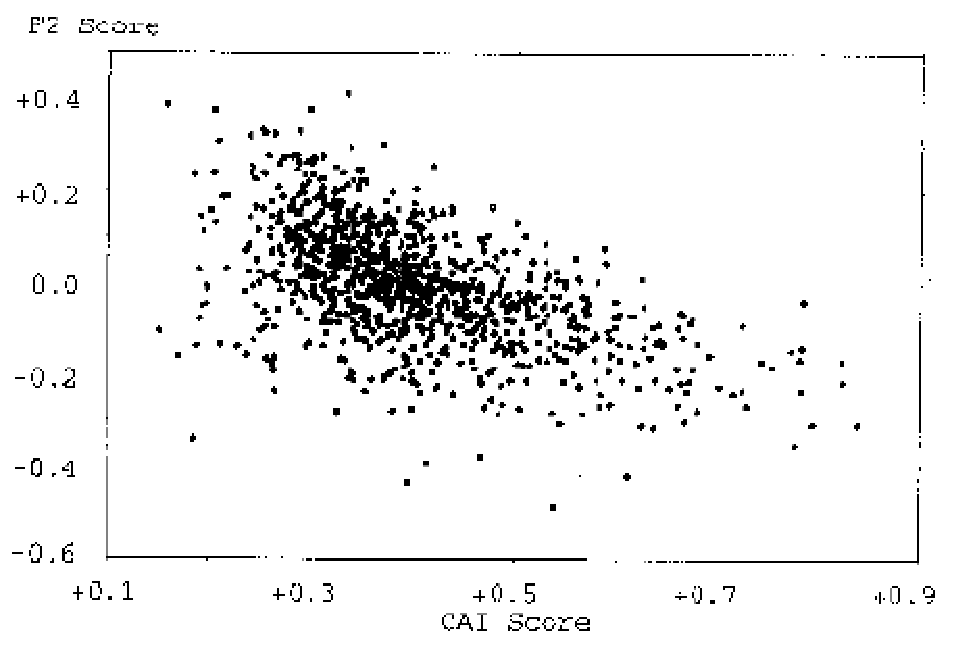
\includegraphics{../figs/lobgau5}
   \end{center}
   \caption{Screenshot of figure 5 from \cite{lobrygautier}. Each point represents
   a protein. This was to show the correlation between the codon adaptation index (CAI Score)
   with the second factor of correspondence analysis at the amino-acid level (F2 Score). Highly
   expressed genes have a high CAI value.
   }
   \label{lobgau5}
\end{figure}


To illustrate the interest of synonymous codon usage analyses, let's use now a more realistic example.
In \cite{lobrygautier} there was an assertion stating that selection for
translation optimisation in \textit{Escherichia coli} was also visible at the amino-acid level.
The argument was in figure 5 of the paper (\textit{cf} fig \ref{lobgau5}), that can be reproduced\footnote{
  the code to reproduce all figures from \cite{lobrygautier} is available at
  \url{http://pbil.univ-lyon1.fr/members/lobry/repro/nar94/}.
} with the following R code:

%
% C'est long celui-la, vaudrait mieux refaire les calculs a partir de ec999, ca illustrerait
% comment on calcule le CAI
%
\begin{Schunk}
\begin{Sinput}
 ec <- read.table(file = "ftp://pbil.univ-lyon1.fr/pub/datasets/NAR94/data.txt", 
     header = TRUE, row.names = 1)
 ec.coa <- dudi.coa(ec, scann = FALSE, nf = 3)
 F2 <- ec.coa$li[, 2]
 tmp <- read.table(file = "ftp://pbil.univ-lyon1.fr/pub/datasets/NAR94/ecoli999.cai")
 cai <- exp(tmp$V2)
 if (cor(cai, F2) > 0) F2 <- -F2
 plot(cai, F2, pch = 20, xlab = "CAI Score", ylab = "F2 Score", 
     main = "Fig 5 from Lobry & Gautier (1994) NAR 22:3174")
\end{Sinput}
\end{Schunk}
\includegraphics{../figs/multivariate-reprolobgau}


So, there was a correlation between the CAI (Codon Adaptation Index \cite{CAI}) and
the second factor for amino-acid composition variability. However, this
is not completely convincing because the CAI is not completely independent
of the amino-acid composition of the protein. Let's use within amino-acid
correspondence analysis to remove the amino-acid effect. Here is a commented
step-by-step analysis:

\begin{Schunk}
\begin{Sinput}
 data(ec999)
 class(ec999)
\end{Sinput}
\begin{Soutput}
[1] "list"
\end{Soutput}
\begin{Sinput}
 names(ec999)[1:10]
\end{Sinput}
\begin{Soutput}
 [1] "ECFOLE.FOLE"     "ECMSBAG.MSBA"    "ECNARZYW-C.NARV" "ECNARZYW-C.NARW"
 [5] "ECNARZYW-C.NARY" "ECNARZYW-C.NARZ" "ECNIRBC.NIRB"    "ECNIRBC.NIRD"   
 [9] "ECNIRBC.NIRC"    "ECNIRBC.CYSG"   
\end{Soutput}
\begin{Sinput}
 ec999[[1]][1:50]
\end{Sinput}
\begin{Soutput}
 [1] "a" "t" "g" "c" "c" "a" "t" "c" "a" "c" "t" "c" "a" "g" "t" "a" "a" "a"
[19] "g" "a" "a" "g" "c" "g" "g" "c" "c" "c" "t" "g" "g" "t" "t" "c" "a" "t"
[37] "g" "a" "a" "g" "c" "g" "t" "t" "a" "g" "t" "t" "g" "c"
\end{Soutput}
\end{Schunk}

This is to load the data from \cite{lobrygautier} which is available as \texttt{ec999}
in the \seqinr{} package. The letters \texttt{ec} are for the bacterium 
\textit{Escherichia coli} and the number \texttt{999} means that there were
$999$ coding sequences available from this species at that time. The class of the
object \texttt{ec999} is a list, which names are the coding sequence names, for instance
the first coding sequence name is 
\texttt{ECFOLE.FOLE}.
Each element of the list is a vector of character, we have listed just above the 50 first
character of the first coding sequence of the list with \texttt{ec999[[1]][1:50]}, we
can see that there is a start codon (ATG) at the beginning of the first coding sequence.

\begin{Schunk}
\begin{Sinput}
 ec999.uco <- lapply(ec999, uco)
 class(ec999.uco)
\end{Sinput}
\begin{Soutput}
[1] "list"
\end{Soutput}
\begin{Sinput}
 class(ec999.uco[[1]])
\end{Sinput}
\begin{Soutput}
[1] "table"
\end{Soutput}
\begin{Sinput}
 ec999.uco[[1]]
\end{Sinput}
\begin{Soutput}
aaa aac aag aat aca acc acg act aga agc agg agt ata atc atg att caa cac cag 
  9   5   2   4   2   8   8   1   0   2   0   4   0   9   8   6   2   3   7 
cat cca ccc ccg cct cga cgc cgg cgt cta ctc ctg ctt gaa gac gag gat gca gcc 
  7   1   1   6   0   1   7   1   4   1   3  13   3  12   3   1   9   1   6 
gcg gct gga ggc ggg ggt gta gtc gtg gtt taa tac tag tat tca tcc tcg tct tga 
  7   5   2   3   0   4   0   5   9   4   0   2   0   2   2   3   2   1   1 
tgc tgg tgt tta ttc ttg ttt 
  1   0   1   1   4   2   3 
\end{Soutput}
\end{Schunk}

This is to compute the codon usage, that is how many times each codon is used
in each coding sequence. Because \texttt{ec999} is a list, we use the function
\texttt{lapply()} to apply the same function, \texttt{uco()}, to all the
elements of the list and we store the result in the object \texttt{ec999.uco}.
The object \texttt{ec999.uco} is a list too, and all its elements belong to
the class table.

\begin{Schunk}
\begin{Sinput}
 df <- as.data.frame(lapply(ec999.uco, as.vector))
 dim(df)
\end{Sinput}
\begin{Soutput}
[1]  64 999
\end{Soutput}
\begin{Sinput}
 df[1:5, 1:5]
\end{Sinput}
\begin{Soutput}
  ECFOLE.FOLE ECMSBAG.MSBA ECNARZYW.C.NARV ECNARZYW.C.NARW ECNARZYW.C.NARY
1           9           15               2               6              23
2           5           18               2               4              16
3           2            8               1               3               4
4           4            3               2               2               4
5           2            3               1               1               0
\end{Soutput}
\end{Schunk}

This is to put the codon usage into a data.frame. Note that the codons are in row
and the coding sequences are in columns. This is more convenient for the following
because groups for within and between analyses are usually handled by row.

\begin{Schunk}
\begin{Sinput}
 row.names(df) <- names(ec999.uco[[1]])
 df[1:5, 1:5]
\end{Sinput}
\begin{Soutput}
    ECFOLE.FOLE ECMSBAG.MSBA ECNARZYW.C.NARV ECNARZYW.C.NARW ECNARZYW.C.NARY
aaa           9           15               2               6              23
aac           5           18               2               4              16
aag           2            8               1               3               4
aat           4            3               2               2               4
aca           2            3               1               1               0
\end{Soutput}
\end{Schunk}

This is to keep a trace of codon names, just in case we would like to re-order
the dataframe \texttt{df}. This is important because we can now play with
the data at will without loosing any critical information. 

\begin{Schunk}
\begin{Sinput}
 ec999.coa <- dudi.coa(df = df, scannf = FALSE)
 ec999.coa
\end{Sinput}
\begin{Soutput}
Duality diagramm
class: coa dudi
$call: dudi.coa(df = df, scannf = FALSE)

$nf: 2 axis-components saved
$rank: 63
eigen values: 0.05536 0.02712 0.02033 0.01884 0.01285 ...
  vector length mode    content       
1 $cw    999    numeric column weights
2 $lw    64     numeric row weights   
3 $eig   63     numeric eigen values  

  data.frame nrow ncol content             
1 $tab       64   999  modified array      
2 $li        64   2    row coordinates     
3 $l1        64   2    row normed scores   
4 $co        999  2    column coordinates  
5 $c1        999  2    column normed scores
other elements: N 
\end{Soutput}
\end{Schunk}

This is to run global correspondence analysis of codon usage.
We have set the \texttt{scannf} parameter to \texttt{FALSE}
because otherwise the eigenvalue bar plot is displayed for the
user to select manually the number of axes to be kept.


\begin{Schunk}
\begin{Sinput}
 facaa <- as.factor(aaa(translate(s2c(c2s(rownames(df))))))
 facaa
\end{Sinput}
\begin{Soutput}
 [1] Lys Asn Lys Asn Thr Thr Thr Thr Arg Ser Arg Ser Ile Ile Met Ile Gln His
[19] Gln His Pro Pro Pro Pro Arg Arg Arg Arg Leu Leu Leu Leu Glu Asp Glu Asp
[37] Ala Ala Ala Ala Gly Gly Gly Gly Val Val Val Val Stp Tyr Stp Tyr Ser Ser
[55] Ser Ser Stp Cys Trp Cys Leu Phe Leu Phe
21 Levels: Ala Arg Asn Asp Cys Gln Glu Gly His Ile Leu Lys Met Phe ... Val
\end{Soutput}
\end{Schunk}

This is to define a factor for amino-acids. The function \texttt{translate()} use by
default the standard genetic code and this is OK for \textit{E. coli}.

\begin{Schunk}
\begin{Sinput}
 ec999.syn <- within(dudi = ec999.coa, fac = facaa, scannf = FALSE)
 ec999.syn
\end{Sinput}
\begin{Soutput}
Within analysis
call: within(dudi = ec999.coa, fac = facaa, scannf = FALSE)
class: within dudi 

$nf (axis saved) : 2
$rank:  43
$ratio:  0.6438642

eigen values: 0.04855 0.0231 0.01425 0.007785 0.006748 ...

  vector length mode    content            
1 $eig   43     numeric eigen values       
2 $lw    64     numeric row weigths        
3 $cw    999    numeric col weigths        
4 $tabw  21     numeric table weigths      
5 $fac   64     numeric factor for grouping

  data.frame nrow ncol content                      
1 $tab       64   999  array class-variables        
2 $li        64   2    row coordinates              
3 $l1        64   2    row normed scores            
4 $co        999  2    column coordinates           
5 $c1        999  2    column normed scores         
6 $ls        64   2    supplementary row coordinates
7 $as        2    2    inertia axis onto within axis
\end{Soutput}
\end{Schunk}

This is to run the synonymous codon usage analysis. The value of the \texttt{ratio} component of
the object \texttt{ec999.syn} shows that most of the variability is at the synonymous
level, a common situation in codon usage studies.

\begin{Schunk}
\begin{Sinput}
 ec999.btw <- between(dudi = ec999.coa, fac = facaa, scannf = FALSE)
 ec999.btw
\end{Sinput}
\begin{Soutput}
Between analysis
call: between(dudi = ec999.coa, fac = facaa, scannf = FALSE)
class: between dudi 

$nf (axis saved) : 2
$rank:  20
$ratio:  0.3561358

eigen values: 0.01859 0.0152 0.01173 0.01051 0.008227 ...

  vector length mode    content      
1 $eig   20     numeric eigen values 
2 $lw    21     numeric group weigths
3 $cw    999    numeric col weigths  

  data.frame nrow ncol content                       
1 $tab       21   999  array class-variables         
2 $li        21   2    class coordinates             
3 $l1        21   2    class normed scores           
4 $co        999  2    column coordinates            
5 $c1        999  2    column normed scores          
6 $ls        64   2    row coordinates               
7 $as        2    2    inertia axis onto between axis
\end{Soutput}
\end{Schunk}

This is to run the non-sysnonymous codon usage analysis, or amino-acid usage analysis.

\begin{Schunk}
\begin{Sinput}
 x <- ec999.syn$co[, 1]
 y <- ec999.btw$co[, 2]
 if (cor(x, y) < 0) y <- -y
 kxy <- kde2d(x, y, n = 100)
 nlevels <- 25
 breaks <- seq(from = min(kxy$z), to = max(kxy$z), length = nlevels + 
     1)
 col <- cm.colors(nlevels)
 image(kxy, breaks = breaks, col = col, xlab = "First synonymous factor", 
     ylab = "Second non-synonymous factor", xlim = c(-0.5, 
         0.5), ylim = c(-0.3, 0.3), las = 1, main = "The second factor for amino-acid variability is\ncorrelated with gene expressivity")
 contour(kxy, add = TRUE, nlevels = nlevels, drawlabels = FALSE)
 box()
 abline(c(0, 1), lty = 2)
 abline(lm(y ~ x))
 legend("topleft", lty = c(2, 1), legend = c("y = x", "y = lm(y~x)"), 
     inset = 0.01, bg = "white")
\end{Sinput}
\end{Schunk}
\includegraphics{../figs/multivariate-vlg9}

This is to plot the whole thing. We have extracted the coding sequences coordinates
on the first synonymous factor and the second non-synonymous factor within
\texttt{x} and \texttt{y}, respectively. Because we have many points, we
use the two-dimensional kernel density estimation provided by the function
\texttt{kde2d()} from package \texttt{MASS}.


%
% Akashi Gojobori
%

\textit{To be completed}

% latex table generated in R 2.8.0 by xtable 1.5-4 package
% Sun Oct 26 18:14:47 2008
\begin{table}[ht]
\begin{center}
\begin{tabular}{rlllrrrl}
  \hline
 & aaa & a & prec & p & h & tot & gc \\
  \hline
1 & Ala & A & pyr & 1 & 5 & 12 & h \\
  2 & Cys & C & 3pg & 7 & 9 & 25 & m \\
  3 & Asp & D & oaa & 1 & 6 & 13 & m \\
  4 & Glu & E & akg & 3 & 6 & 15 & m \\
  5 & Phe & F & 2 pep, eryP & 13 & 19 & 52 & l \\
  6 & Gly & G & 3pg & 2 & 5 & 12 & h \\
  7 & His & H & penP & 20 & 9 & 38 & m \\
  8 & Ile & I & pyr, oaa & 4 & 14 & 32 & l \\
  9 & Lys & K & oaa, pyr & 4 & 13 & 30 & l \\
  10 & Leu & L & 2 pyr, acCoA & 3 & 12 & 27 & l \\
  11 & Met & M & oaa, Cys, -pyr & 10 & 12 & 34 & m \\
  12 & Asn & N & oaa & 3 & 6 & 15 & l \\
  13 & Pro & P & akg & 4 & 8 & 20 & h \\
  14 & Gln & Q & akg & 4 & 6 & 16 & m \\
  15 & Arg & R & akg & 11 & 8 & 27 & h \\
  16 & Ser & S & 3pg & 2 & 5 & 12 & m \\
  17 & Thr & T & oaa & 3 & 8 & 19 & m \\
  18 & Val & V & 2 pyr & 2 & 11 & 23 & m \\
  19 & Trp & W & 2 pep, eryP, PRPP, -pyr & 28 & 23 & 74 & m \\
  20 & Tyr & Y & eryP, 2 pep & 13 & 18 & 50 & l \\
   \hline
\end{tabular}
\caption{Aerobic cost of amino-acids in \textit{Escherichia coli} and G+C classes to be loaded with \texttt{data(aacost).}}
\label{aacost}
\end{center}
\end{table}



\section*{Session Informations}

\begin{scriptsize}

This part was compiled under the following \Rlogo{}~environment:

\begin{itemize}
  \item R version 2.9.0 (2009-04-17), \verb|i386-apple-darwin8.11.1|
  \item Locale: \verb|C|
  \item Base packages: base, datasets, grDevices, graphics, grid,
    methods, stats, utils
  \item Other packages: MASS~7.2-46, XML~2.3-0, ade4~1.4-11,
    ape~2.3, grImport~0.4-3, quadprog~1.4-11, seqinr~2.0-3,
    tseries~0.10-18, xtable~1.5-5, zoo~1.5-5
  \item Loaded via a namespace (and not attached): gee~4.13-13,
    lattice~0.17-22, nlme~3.1-90, tools~2.9.0
\end{itemize}
There were two compilation steps:

\begin{itemize}
  \item \Rlogo{} compilation time was: Thu Apr 23 11:56:34 2009
  \item \LaTeX{} compilation time was: \today
\end{itemize}

\end{scriptsize}

% END - DO NOT REMOVE THIS LINE

%%%%%%%%%%%%  BIBLIOGRAPHY %%%%%%%%%%%%%%%%%
\clearpage
\addcontentsline{toc}{section}{References}
\bibliographystyle{plain}
\bibliography{../config/book}
\end{document}
